\subsection{DIAGRAMM}
\begin{figure}[H]
  \centering
  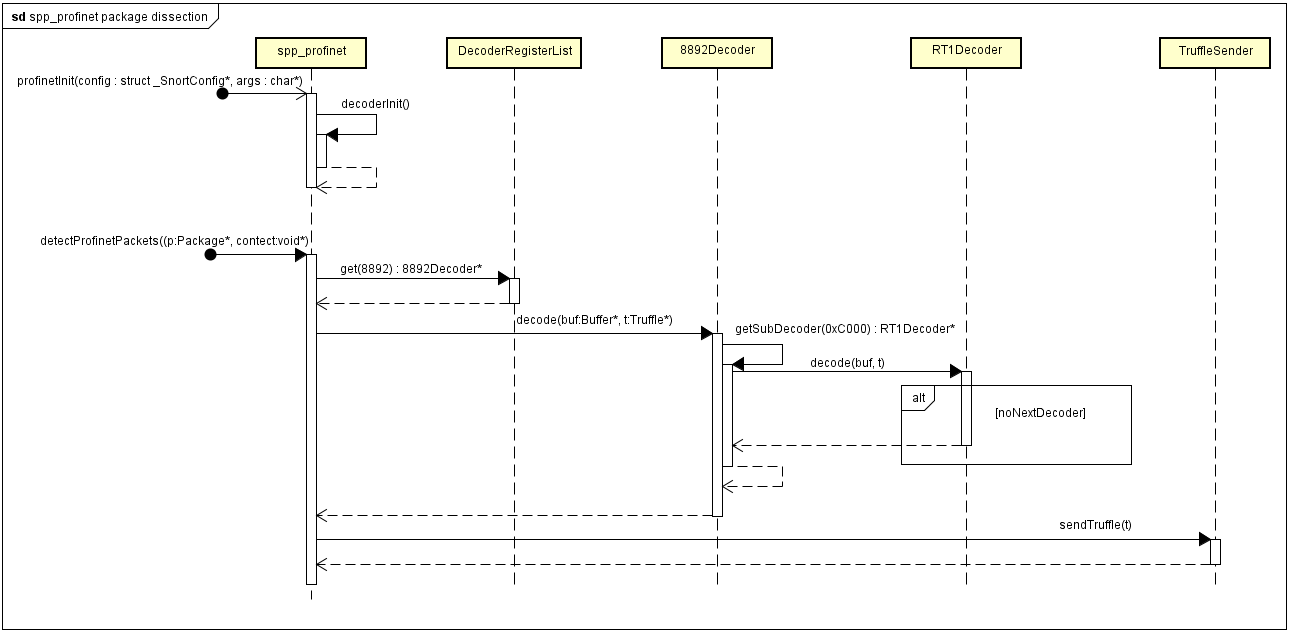
\includegraphics[width=\textwidth]{../diagramimages/spp-profinet-package-dissection.png}
  \caption[Sequenzdiagramm DIAGRAMM]{Sequenzdiagramm DIAGRAMM}
\end{figure}

In diesem Diagramm wird die Ausführung des LoadSnapshotCommand dargestellt. Erstellt wird der Command von der View, wenn der Benutzer versucht Replays anzusehen. Der Command ruft load() im dem ReplayLogLoadService auf. Dieser nimmt das übergebene Instant an und deserialisiert damit den ReplayLog, der den Graphen und die Commands liefert. Im Proxy, der für den Replaygraph zuständig ist, wird der geladene Graph referenziert. Danach wird im ReplayLogLoadService das play-Flag gesetzt (da Service im eigenen Thread läuft, was zwecks besserer Übersicht ausgelassen wurde) und im NetworkGraphSwitch stellt man den
aktuell dargestellten Graphen auf Replaygraph um.